
\section{Introduction to IEC 61499 Portability Challenges}

The IEC 61499 standard was developed to address the increasing demands for decentralized control and the exponential growth of control complexity in industrial automation systems. Its primary goal was to establish an open, component-oriented, and platform-independent development framework to improve the reusability, reconfigurability, interoperability, portability, and distribution of control software for complex distributed systems. However, despite these ambitious objectives, the reality of IEC 61499 implementation has revealed significant challenges in achieving true portability across different vendor platforms.

\subsection{The Promise and Reality of IEC 61499 Portability}

The IEC 61499 standard provides a standardized XML format for data exchange between different development environments, theoretically enabling seamless portability of function blocks across various vendor platforms. This standardization was intended to eliminate vendor lock-in and facilitate the development of distributed control systems that could operate across heterogeneous hardware and software environments. The technology has been effectively used in implementing Intelligent Mechatronic Components and engineering processes using multiple commercial tools and hardware platforms.

However, the practical implementation of IEC 61499 portability has encountered significant obstacles. While the file exchange format is standardized, it is currently interpreted differently across various vendors, and the execution semantics vary considerably among different runtime environments. This divergence in interpretation and execution behavior has created a situation where migrating programs from one IEC 61499 platform to another can introduce errors that are difficult to detect but could potentially lead to damage to humans or physical equipment.

\subsection{Vendor-Specific Execution Semantics}

The fundamental challenge lies in the fact that the IEC 61499 language semantics is not formally specified and is subject to interpretation by different vendors. This has led to the emergence of different execution semantics across various runtime environments, which can significantly affect the behavior of cyber-physical systems. For example, when an identical function block is executed on different runtime environments, it may exhibit different behaviors due to variations in event processing order and timing, state transition mechanisms, data type handling and boundary conditions, algorithm execution semantics, and communication and synchronization protocols.

These semantic variations pose a significant challenge for developers who need to ensure that their control applications behave consistently across different platforms. The lack of standardized execution semantics means that even syntactically equivalent IEC 61499 applications may behave differently when deployed on different runtime environments.

\subsection{The Need for Systematic Testing Approaches}

Given these challenges, it becomes crucial to thoroughly test IEC 61499 applications on each relevant target platform before deploying them to real-world systems. Traditional testing approaches that rely on manual verification or platform-specific testing frameworks are insufficient for addressing the cross-platform compatibility issues inherent in IEC 61499 applications.

A platform-independent test specification has the potential to greatly reduce the effort involved in validating IEC 61499 applications across multiple platforms. Such an approach would enable developers to systematically evaluate the behavior of function blocks across different runtime environments, identify and document vendor-specific execution differences, and ensure consistent behavior of control applications regardless of the target platform. This systematic approach would significantly reduce the time and effort required for cross-platform validation while improving the reliability and safety of distributed control systems.

The development of comprehensive testing methodologies for IEC 61499 applications is therefore essential for realizing the full potential of the standard in industrial automation systems.

\section{Comprehensive Test Function Block Development}

To address the portability challenges in IEC 61499 applications, a systematic approach to testing function blocks across different development and runtime environments is required. This approach involves the development of specialized test function blocks that can validate various aspects of IEC 61499 compliance and portability.

\subsection{Data Type Testing Framework}

The foundation of any IEC 61499 testing framework lies in the comprehensive validation of data type support and handling across different platforms. Data types in IEC 61499 include bit string types (BOOL, BYTE, WORD, DWORD, LWORD), integer types (SINT, INT, DINT, LINT, USINT, UINT, UDINT, ULINT), real types (REAL, LREAL), string types (STRING), and various time-related types (TIME, DATE, TIME\_OF\_DAY, DATE\_AND\_TIME).

\begin{figure}[!htbp]
    \centering
    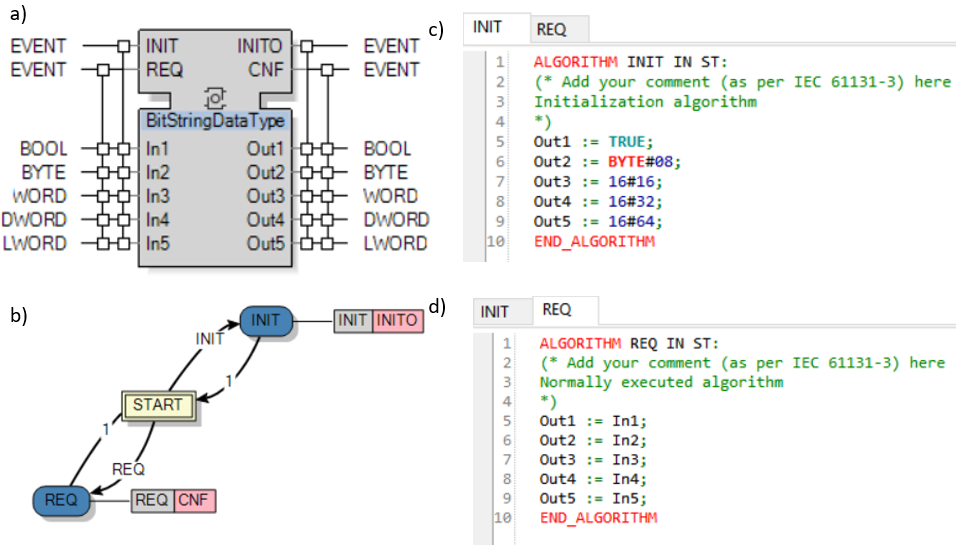
\includegraphics[width=0.8\columnwidth]{MX_Papers/Paper8/Figures/BSDT.PNG}
    \caption{BitStringDataType Function Block: Interface, Execution Control Chart (ECC), and algorithms for testing bit string data type support across IEC 61499 platforms.}
    \label{fig:bitstring_test}
\end{figure}

The BitStringDataType function block serves as a comprehensive testing tool for validating bit string data type support. This function block implements a systematic testing procedure involving two primary events: INIT and REQ. When the INIT event is triggered, the function block sets output values to predefined constants, allowing verification that the platform correctly handles each supported bit string data type. The REQ event, on the other hand, tests the dynamic processing of input data by ensuring that output values correspond exactly to input values, with the CNF event confirming successful completion.

Similarly, the IntegerDataType function block validates support for all integer data types defined in the IEC 61499 standard. This function block tests both the initialization of integer values and the dynamic processing of integer data, ensuring that platforms correctly handle signed and unsigned integers of various bit lengths. The testing procedure verifies that output values match expected results for both predefined constants and dynamic input values.

\begin{figure}[!htbp]
    \centering
    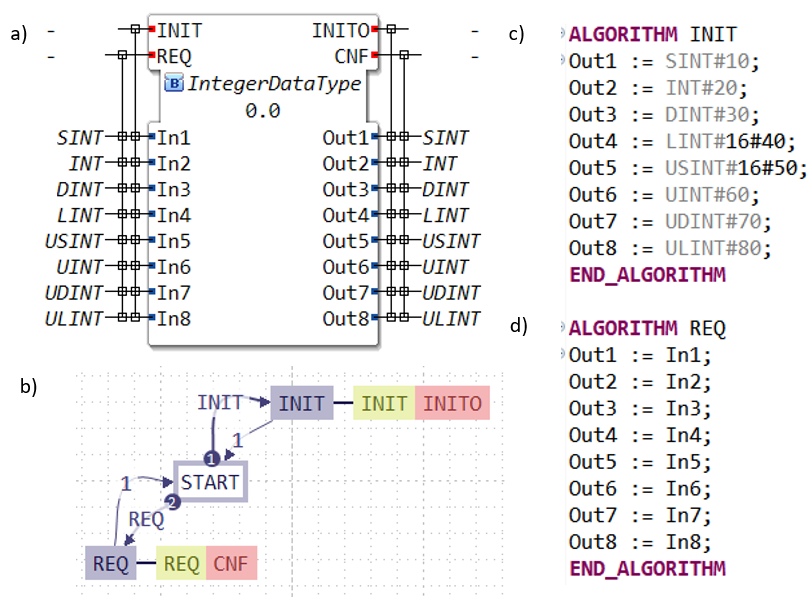
\includegraphics[width=0.8\columnwidth]{MX_Papers/Paper8/Figures/IDT.PNG}
    \caption{IntegerDataType Function Block: Comprehensive testing of integer data type support including signed and unsigned variants across different bit lengths.}
    \label{fig:integer_test}
\end{figure}

The RealDataType function block focuses on validating floating-point number handling, which is critical for many industrial control applications. This function block tests both REAL and LREAL data types, ensuring that platforms correctly handle precision and range requirements for floating-point arithmetic operations.

String data type testing is implemented through the StringDataType function block, which validates the handling of character strings across different platforms. This is particularly important for applications that require human-readable output or configuration data.

Time-related data types are tested through specialized function blocks (TimeDataType, DateDataType, TimeOfDayDataType, and DateAndTimeOfDayDataType) that validate the correct handling of temporal information, which is essential for real-time control applications.

\subsection{Boundary Condition Validation}

Beyond basic data type support, it is crucial to validate how platforms handle boundary conditions and extreme values. The BoundCheckTest function block provides comprehensive testing of boundary conditions for all supported data types.

\begin{figure}[!htbp]
    \centering
    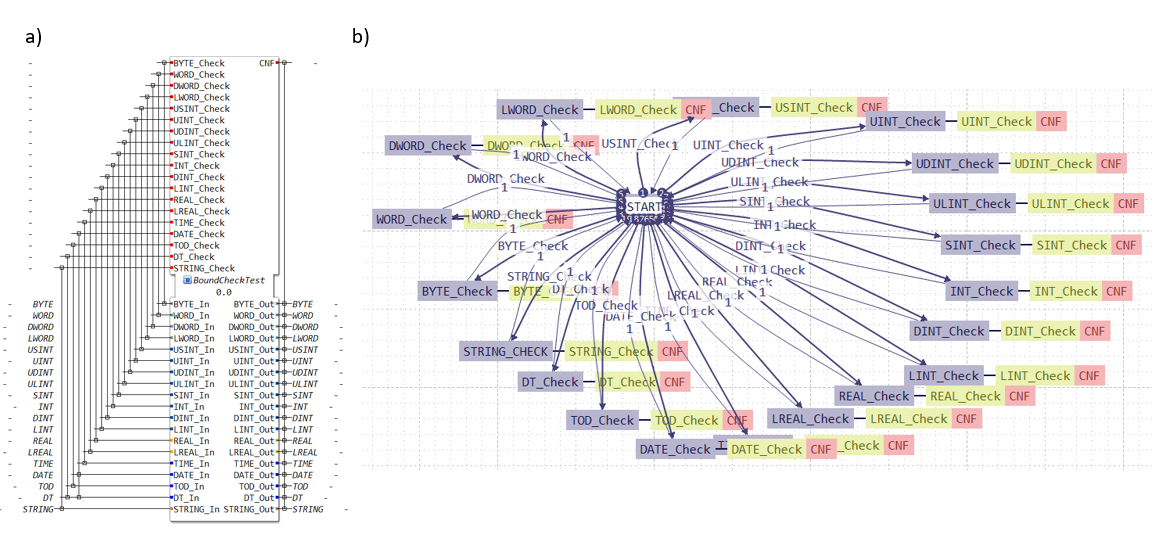
\includegraphics[width=0.9\columnwidth]{MX_Papers/Paper8/Figures/BCT4Diac.PNG}
    \caption{BoundCheckTest Function Block: Interface and Execution Control Chart for validating boundary conditions and extreme values across all IEC 61499 data types.}
    \label{fig:boundary_test}
\end{figure}

This function block tests the maximum and minimum values for each data type, ensuring that platforms can handle extreme values without errors or unexpected behavior. The testing procedure involves providing input values at the boundaries of each data type's range and verifying that the platform correctly processes these values and produces expected output results.

Boundary condition testing is particularly important for industrial control applications where sensor readings or control outputs may reach extreme values. Proper handling of these conditions is essential for system reliability and safety.

\subsection{Standard Function and Composite Block Testing}

The StandardFunctionTest function block evaluates support for IEC 61499 standard functions and their corresponding associations with input values. This function block is capable of testing over 75 standard functions by providing specific events for testing each function, which trigger the corresponding testing algorithm for that particular function.

\begin{figure}[!htbp]
    \centering
    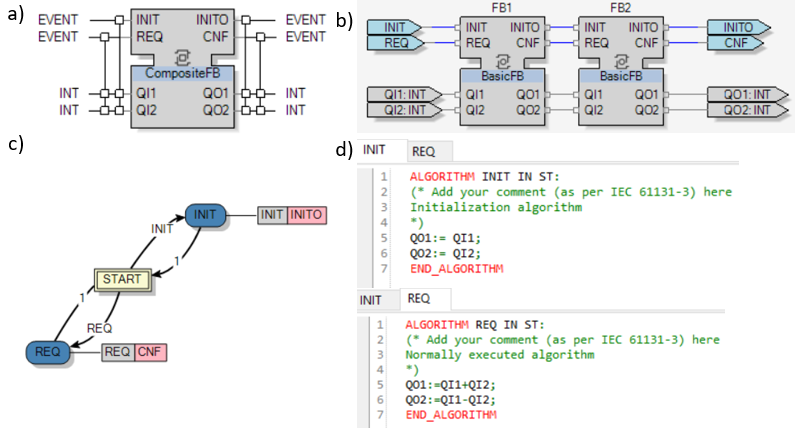
\includegraphics[width=0.8\columnwidth]{MX_Papers/Paper8/Figures/CFBTest.PNG}
    \caption{Composite Function Block Testing: Interface, connection diagram, and algorithms for validating composite function block support across platforms.}
    \label{fig:composite_test}
\end{figure}

For example, the Multiplexer (MUX) function can be tested by triggering the MUX\_Func event and verifying that the output value matches the expected result. This function is used to select one of several input signals based on an index value, and proper implementation is crucial for many control applications.

The CompositeBlockTest function block validates the functionality of composite function block support, which is essential for building complex control applications. This function block tests the initialization and execution of composite blocks, ensuring that they correctly handle input/output relationships and event processing.

\subsection{Adapter and Interface Testing}

Adapter support is a critical aspect of IEC 61499 portability, as adapters enable the connection of function blocks with different interfaces. The AdapterTest composite function block provides comprehensive testing of adapter functionality.

\begin{figure}[!htbp]
    \centering
    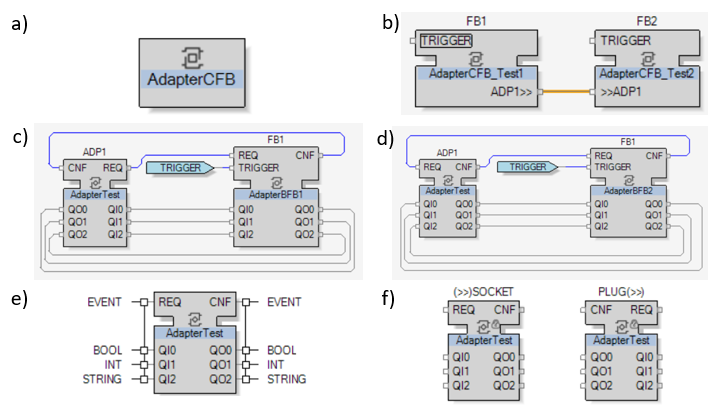
\includegraphics[width=0.8\columnwidth]{MX_Papers/Paper8/Figures/AdapterCFB.PNG}
    \caption{Adapter Testing Framework: Function block interface and structure for validating adapter support and interface compatibility across IEC 61499 platforms.}
    \label{fig:adapter_test}
\end{figure}

This function block consists of two basic function blocks (AdapterBFB1 and AdapterBFB2) connected through an adapter. The testing procedure validates that input values from one function block are correctly transferred to the other through the adapter interface, ensuring that adapter functionality works consistently across different platforms.

Adapter testing is particularly important for distributed control systems where function blocks developed by different vendors or teams need to communicate effectively.

\section{Model-Based Testing Methodologies}

Traditional manual testing approaches for IEC 61499 function blocks are time-consuming and error-prone, especially when dealing with cross-platform compatibility issues. Model-based testing methodologies offer a more systematic and automated approach to function block validation.

\subsection{Service Sequence Models as Test Specifications}

Service sequence models provide a standardized way to specify the expected input/output behavior of IEC 61499 function blocks. These models define the expected event occurrences, input values, and expected output values for each test scenario, making them ideal for automated test generation and execution.

\begin{figure}[!htbp]
    \centering
    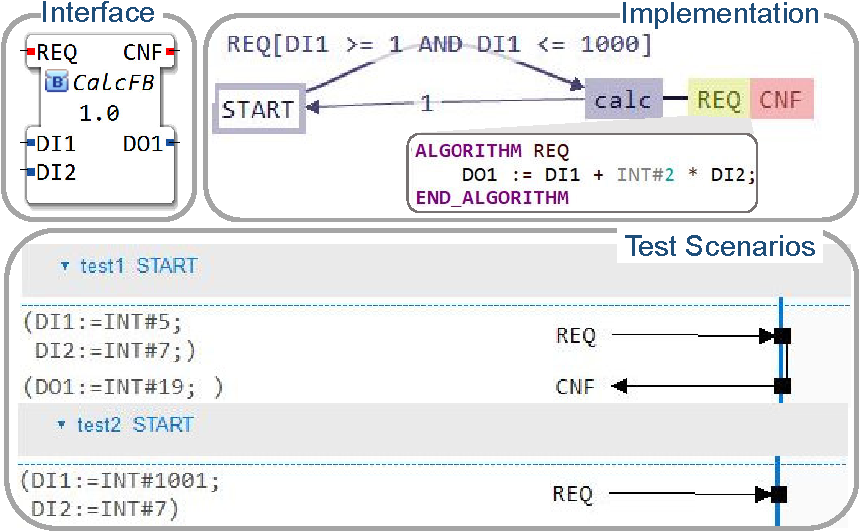
\includegraphics[width=0.75\columnwidth]{MX_Papers/Paper9/Figures/running_example-crop.pdf}
    \caption{Service Sequence Model Example: Function block interface, state diagram, and service sequences defining test scenarios for a simple calculation function block.}
    \label{fig:service_sequence}
\end{figure}

Service sequences can be specified manually for test-driven development or derived from existing implementations using model execution frameworks. This flexibility allows developers to create comprehensive test suites that cover both normal operation and edge cases.

The use of service sequences as test specifications provides several advantages including standardized representation of test scenarios, support for both manual and automated test generation, clear documentation of expected behavior, facilitation of regression testing, and platform-independent test specification.

\subsection{Test-Driven Development for Function Blocks}

Test-driven development (TDD) is a software development methodology that emphasizes writing tests before implementing functionality. This approach is particularly valuable for IEC 61499 function block development, as it helps ensure that the implemented behavior matches the specified requirements from the beginning.

The TDD process for IEC 61499 function blocks involves the following steps:

\begin{enumerate}
    \item Create a new function block type (FBT) with the desired interface
    \item Specify test cases as service sequence models
    \item Implement the desired functionality
    \item Generate test applications from the specifications
    \item Execute tests to validate the implementation
\end{enumerate}

This approach helps identify implementation issues early in the development process and ensures that function blocks behave consistently across different platforms.

\begin{figure}[!htbp]
    \centering
    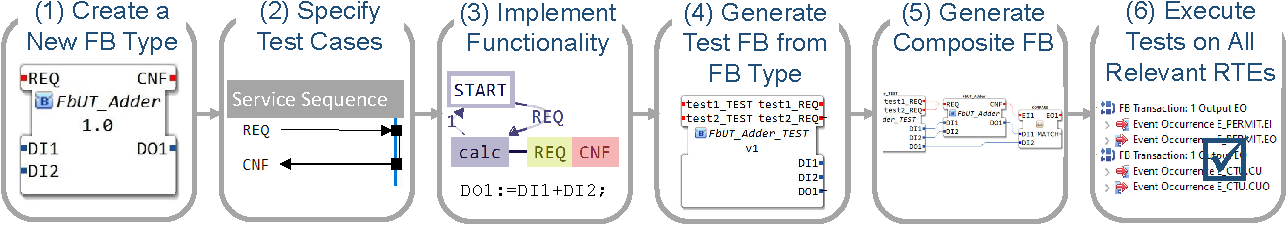
\includegraphics[width=0.85\textwidth]{MX_Papers/Paper9/Figures/process-crop.pdf}
    \caption{Test-Driven Development Process: Overview of the systematic approach for testing function blocks across various software platforms using service sequence models.}
    \label{fig:tdd_process}
\end{figure}

\subsection{Automated Test Generation from Specifications}

The transformation of service sequence models into executable test applications is a key component of model-based testing methodologies. This process involves the application of transformation rules that convert high-level test specifications into IEC 61499-compliant test function blocks.

\begin{figure}[!htbp]
    \centering
    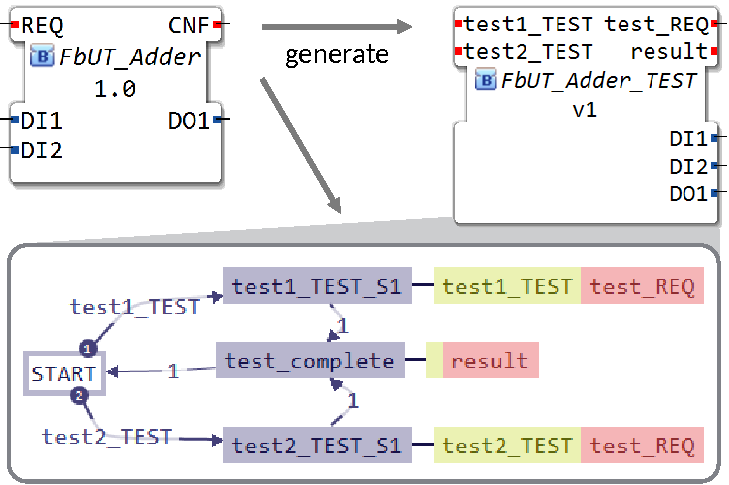
\includegraphics[width=0.8\columnwidth]{MX_Papers/Paper9/Figures/testFB-crop.pdf}
    \caption{Automated Test Generation: Creating test function blocks from service sequence models using transformation rules and automated code generation.}
    \label{fig:test_generation}
\end{figure}

The transformation rules ensure that each service sequence results in a corresponding input event, output events are properly mapped to function block interfaces, data values are set according to service specifications, state diagrams reflect the expected behavior, and test results are properly captured and reported.

This automated approach significantly reduces the manual effort required for test development while ensuring consistency and completeness of test coverage.

\subsection{Transformation Rules and Implementation}

The implementation of transformation rules for automated test generation involves several key principles:

\begin{enumerate}
    \item \textbf{One Input Event per Service Sequence}: Every service sequence must result in a corresponding input event at the test function block, with the event name reflecting the associated sequence.
    
    \item \textbf{One Output Event per Input Event}: The test function block requires one output event for each input event of the function block under test.
    
    \item \textbf{One Output Event for Comparison}: A single output event represents the completion of a test sequence and provides the test result.
    
    \item \textbf{One Data Output per Data Pin}: All input and output data pins of the function block under test are exposed as output pins in the test function block.
    
    \item \textbf{Values Set According to Service Specification}: Data output values are set based on the service sequence specification, ensuring accurate test execution.
    
    \item \textbf{One State per Transaction}: The state diagram of the test function block has one state per transaction, with each state having an algorithm that updates data outputs.
    
    \item \textbf{Output Event upon Test Completion}: The state diagram ensures that the completion event is sent after finishing a sequence.
\end{enumerate}

These transformation rules provide a systematic approach to converting service sequence models into executable test applications, ensuring that the generated tests accurately reflect the intended test scenarios.

\section{Cross-Platform Test Application Architecture}

The development of portable test applications that can execute across different IEC 61499 runtime environments is essential for comprehensive cross-platform validation. These applications must be designed to work with any IEC 61499-compliant platform while providing accurate and reliable test results.

\subsection{Test Signal Generation and Execution}

The core of any cross-platform test application is the test signal generator, which is responsible for providing the necessary events and data to the function block under test. This component generates input signals based on the service model and supplies the required events and data to the function block under test.

\begin{figure}[!htbp]
    \centering
    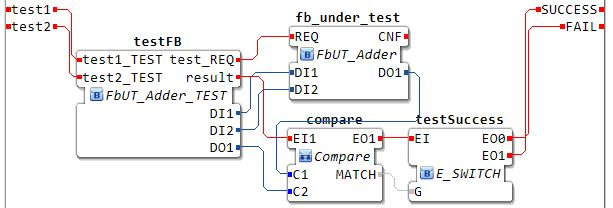
\includegraphics[width=0.8\columnwidth]{MX_Papers/Paper9/Figures/compositeFb.JPG}
    \caption{Composite Test Application: Function block encapsulating the test application with connections between test signal generator, function block under test, and result validation components.}
    \label{fig:composite_test_app}
\end{figure}

The test signal generator must generate appropriate input events based on service sequence specifications, provide correct data values for each test scenario, and notify the test application of expected output events.
    \item Supply expected output values for result comparison
    \item Handle timing requirements for test execution
\end{itemize}

This component ensures that the function block under test receives the correct stimuli to execute the intended test scenarios.

\subsection{Result Comparison and Validation}

The matcher component is responsible for comparing the execution results of the function block under test with the expected results provided by the test signal generator. This component plays a crucial role in determining whether a test passes or fails.

The matcher must receive expected events and data values from the signal generator, compare them with actual events and data received from the function block under test, determine whether the test passed or failed, provide detailed information about any discrepancies, and handle timing issues and synchronization.

The comparison process must be robust enough to handle minor variations in timing and implementation details while still detecting significant behavioral differences.

\subsection{Portable Test Application Design}

The test application is realized as a composite function block that encapsulates all the testing components. This design ensures that the entire test application can be ported to different IEC 61499 platforms as a single unit.

\begin{figure}[!htbp]
    \centering
    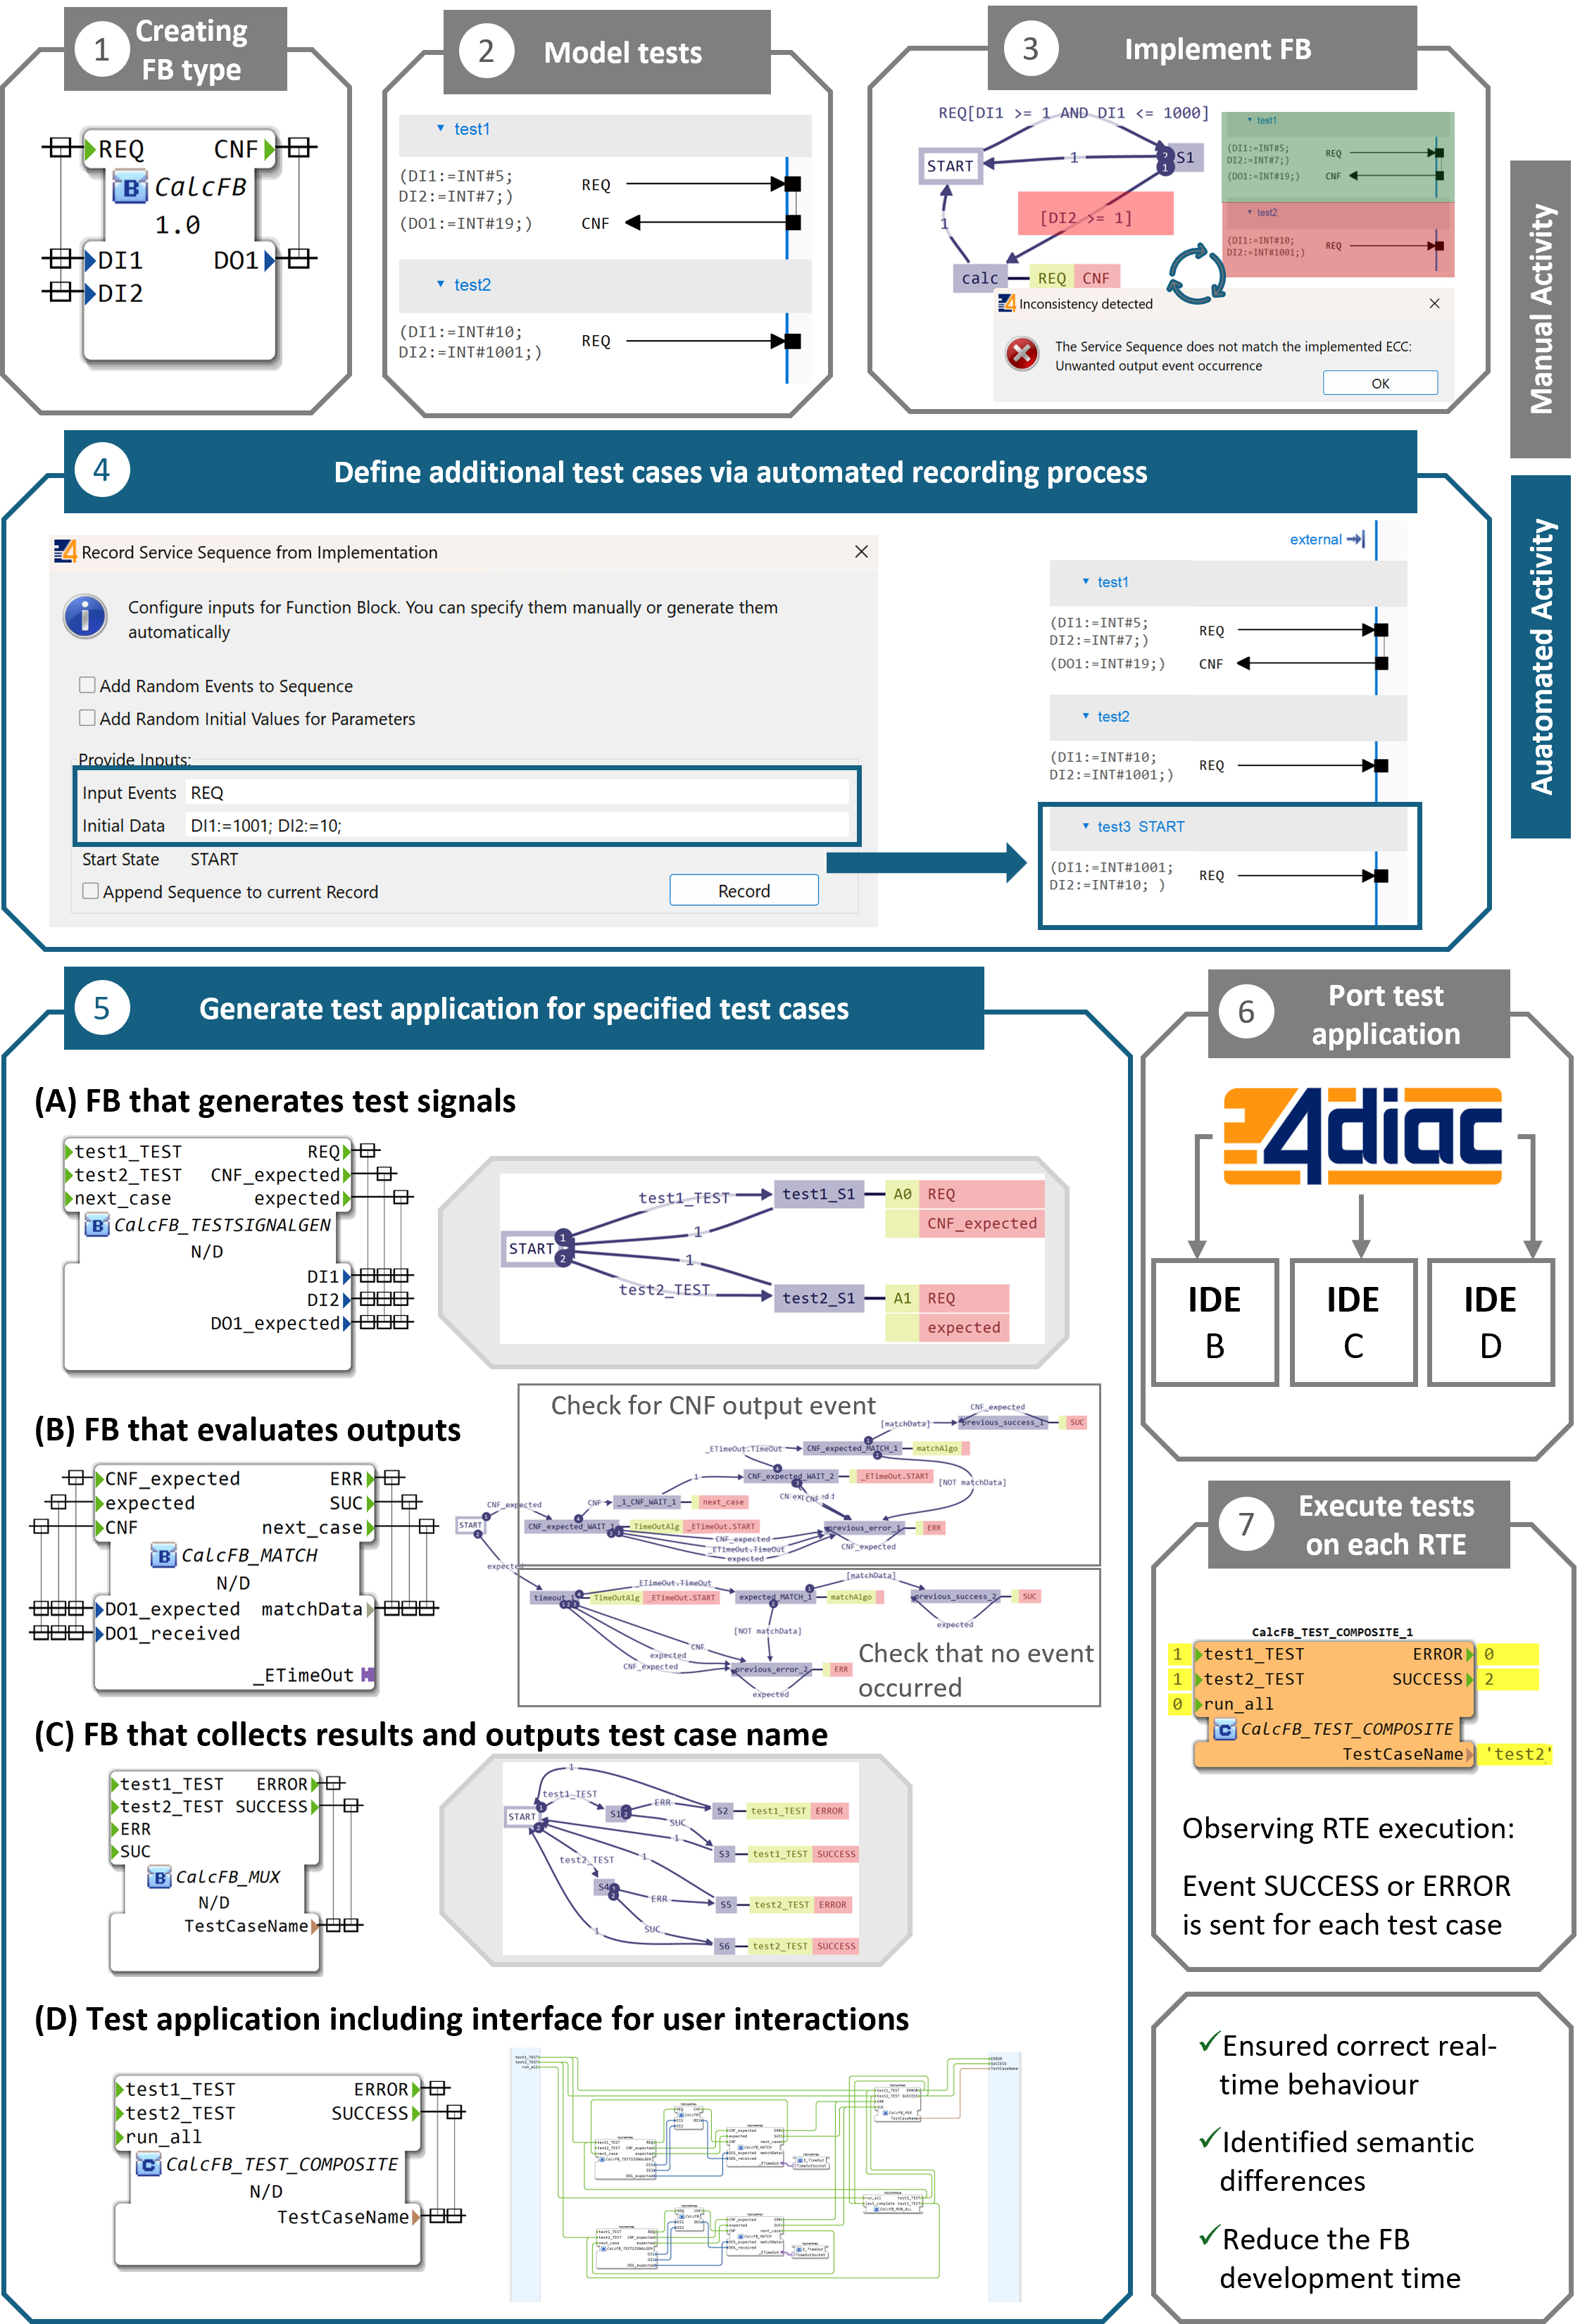
\includegraphics[width=0.85\textwidth]{MX_Papers/Paper10/Figures/methodology_complete.png}
    \caption{Cross-Platform Testing Methodology: Seven-step process for testing function blocks across various software platforms, showing both automated and manual development phases.}
    \label{fig:cross_platform_methodology}
\end{figure}

The composite function block design provides several advantages including portability, where the entire test application can be moved between platforms; encapsulation, where all testing logic is contained within a single function block; simplicity, where the interface is simplified to basic event triggers; flexibility, where individual test cases can be executed separately or in sequence; and reliability, where the internal state is managed consistently across platforms.

The test application includes an additional event pin "run\_all" that allows execution of all test cases sequentially based on a single event trigger, providing convenience for comprehensive testing.

\subsection{Tool Support and Automation}

Sophisticated tool support is essential for automating the test generation and execution process. The Eclipse 4diac IDE provides comprehensive support for specifying service sequences and simulating their results.

\begin{figure}[!htbp]
    \centering
    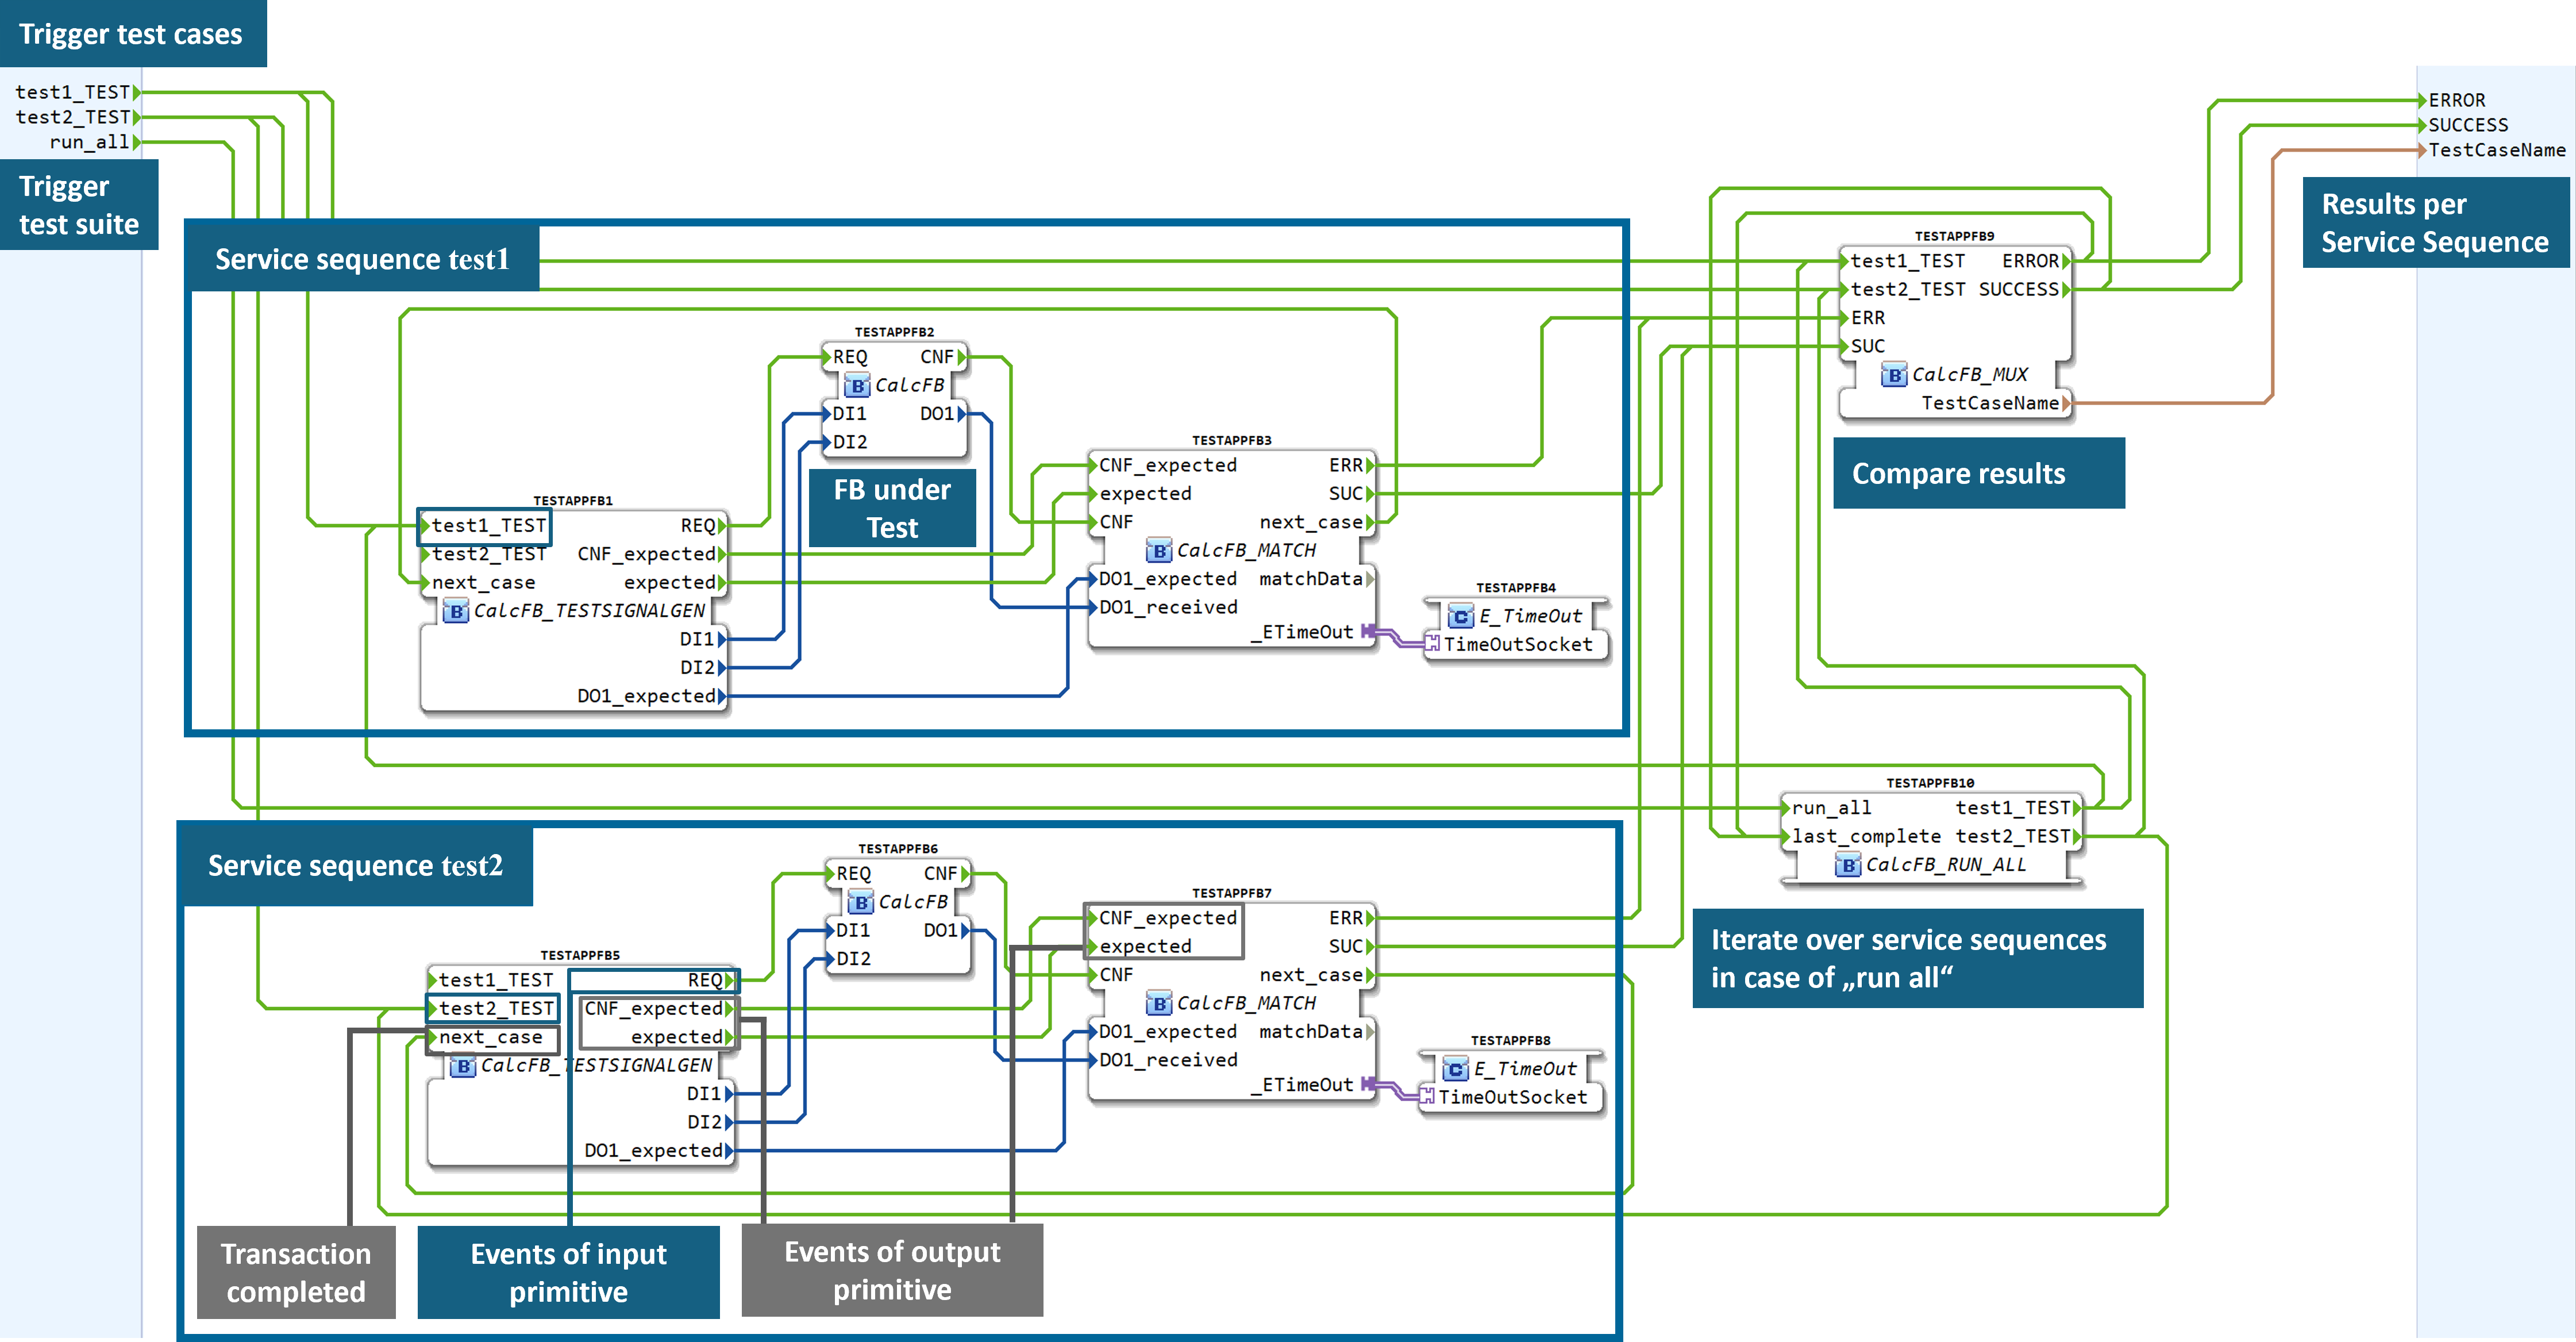
\includegraphics[width=\linewidth]{MX_Papers/Paper10/Figures/generation_rules.png}
    \caption{Test Application Generation: Automated generation of test applications from service sequence models, showing the relationship between service models and generated test components.}
    \label{fig:generation_rules}
\end{figure}

The tool support includes service sequence editors with graphical and textual interfaces for creating service sequence models, a model interpreter framework for executing and validating service sequences, automated test generators for creating test function blocks from service models, result analyzers for analyzing and reporting test results, and export/import capabilities for porting test applications between platforms.

This tool support significantly reduces the manual effort required for test development while ensuring consistency and accuracy in the generated test applications.

\section{Real-World Validation and Case Studies}

The effectiveness of cross-platform testing methodologies must be validated through real-world case studies that demonstrate their applicability to industrial control systems. The processing station case study provides a comprehensive example of how these methodologies can be applied to complex, multi-component control systems.

\subsection{Processing Station Control System}

The processing station represents a realistic industrial control application that demonstrates the complexity and challenges of cross-platform IEC 61499 development. This system consists of several mechatronic components, including a table, tester, and drill component, each equipped with its own control devices.

\begin{figure}[!htbp]
    \centering
    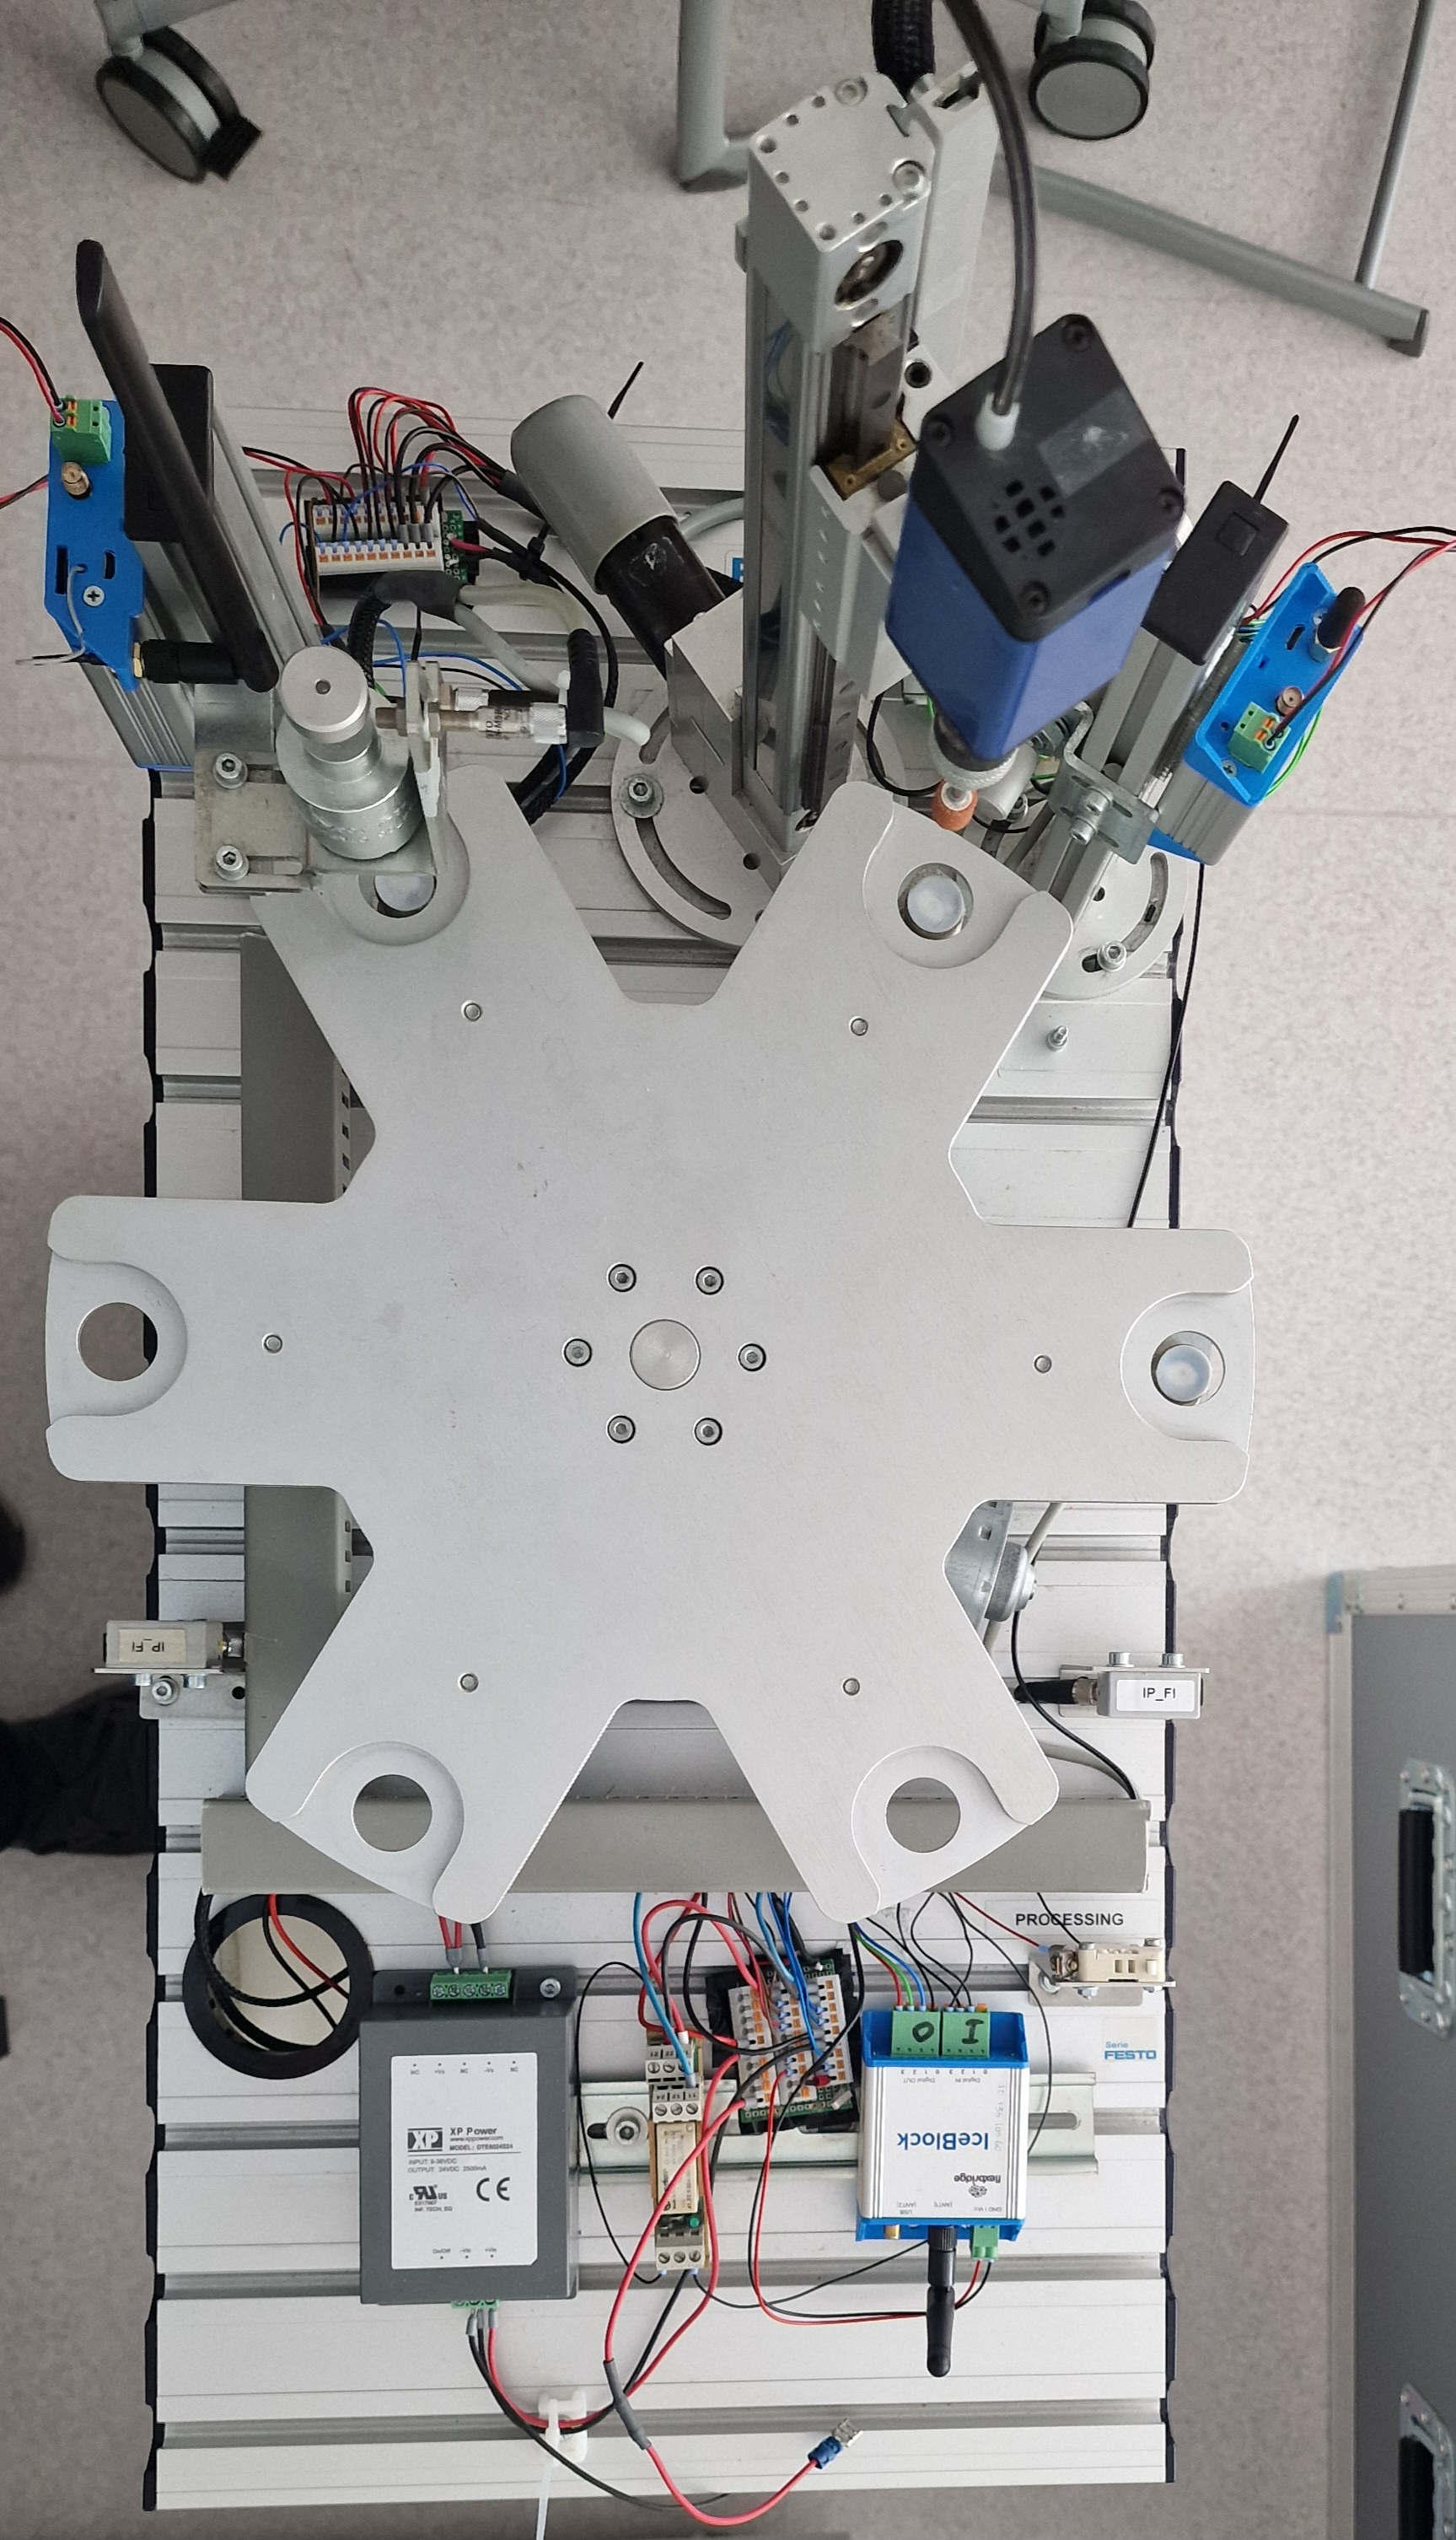
\includegraphics[width=0.5\linewidth]{MX_Papers/Paper10/Figures/processingStation.jpg}
    \caption{Processing Station: Physical layout of the industrial control system used for validating cross-platform testing methodologies.}
    \label{fig:processing_station}
\end{figure}

The processing station operates through a coordinated sequence of operations:

\begin{enumerate}
    \item The table rotates to position material under the tester component
    \item The tester checks whether the material has been drilled
    \item If necessary, the drill component processes the material
    \item The cycle repeats for continuous operation
\end{enumerate}

This system is implemented using IEC 61499 function blocks following the "Chain of Actions" design pattern, which provides a structured approach to coordinating multiple control components.

\subsection{Table Control: Rotation Management}

The TableControl function block network is responsible for managing the rotational movement of the table component. This system must ensure precise positioning while handling various operational scenarios and potential failure conditions.

\begin{figure}[!htbp]
    \centering
    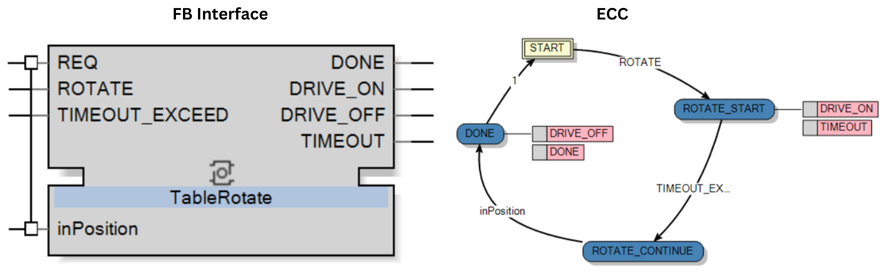
\includegraphics[width=0.99\linewidth]{MX_Papers/Paper10/Figures/TableRotate.png}
    \caption{TableRotate Function Block: Interface, state diagram, and test cases for validating table rotation control across different platforms.}
    \label{fig:table_rotate}
\end{figure}

The TableRotate function block encapsulates the core control logic for table rotation, managing starting and stopping rotation movements, monitoring position feedback, handling timeout conditions, and ensuring safe operation under various conditions.

The state diagram implements a robust control strategy that transitions between START, ROTATE\_START, ROTATE\_CONTINUE, and DONE states based on events and position feedback. This design ensures that the table can be accurately positioned while handling potential sensor failures or timing issues.

Test scenarios for the TableRotate function block include both normal operation and edge cases, such as timeout handling and position sensor failures. These tests validate that the function block behaves correctly across different runtime environments.

\subsection{Tester Control: Inspection Logic}

The TesterControl function block network manages the inspection process for detecting holes in workpieces. This system must ensure that workpieces are not drilled multiple times and that the drilling process is properly verified.

\begin{figure}[!htbp]
    \centering
    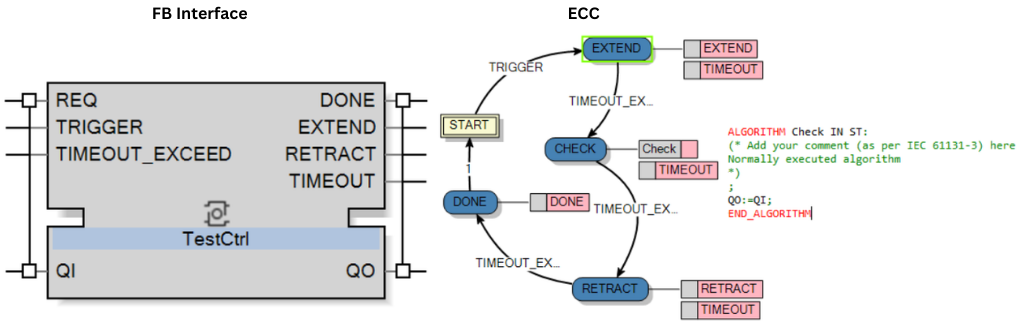
\includegraphics[width=0.99\linewidth]{MX_Papers/Paper10/Figures/TestCtrl.png}
    \caption{TestCtrl Function Block: Interface, state diagram, and timeout test case for validating inspection control logic across platforms.}
    \label{fig:test_ctrl}
\end{figure}

The TestCtrl function block manages the sequence of extending, checking, and retracting the inspection probe, while handling timeout conditions that may occur during the inspection process. The function block transitions through EXTEND, CHECK, RETRACT, and DONE states based on sensor feedback and timing requirements.

Test cases for the TestCtrl function block include scenarios for successful inspection, timeout conditions, and sensor failure handling. These tests ensure that the inspection logic works correctly across different platforms and can handle various operational conditions.

\subsection{Drill Control: Processing Operations}

The DrillControl function block network orchestrates the drilling process, managing both the vertical movement of the drill and the rotation of the drill motor. This system must ensure precise control of drilling operations while maintaining safety and quality requirements.

\begin{figure}[!htbp]
    \centering
    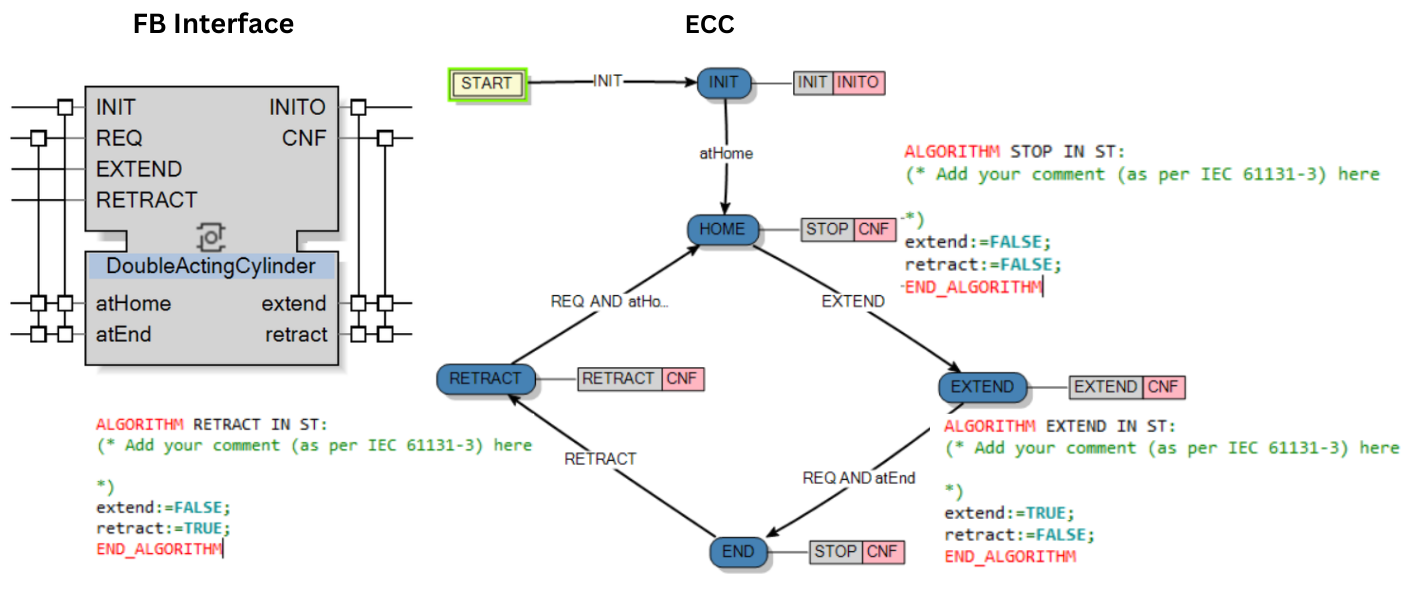
\includegraphics[width=0.99\linewidth]{MX_Papers/Paper10/Figures/DoubleActingCylinderV2.png}
    \caption{Double Acting Cylinder Function Block: Interface, state diagram, and test cases for validating drill control operations across platforms.}
    \label{fig:double_acting_cylinder}
\end{figure}

The DoubleActingCylinder function block controls the bidirectional motion of the drill, managing extension (downward movement) and retraction (upward movement) operations. This function block ensures precise control of the drilling process through proper state management and position feedback.

Test scenarios for the DoubleActingCylinder function block include normal drilling operations, emergency stop conditions, and position sensor failures. These tests validate that the drilling control logic works correctly across different runtime environments.

\subsection{Semantic Execution Differences}

The case study revealed significant semantic execution differences between different IEC 61499 runtime environments, particularly between Eclipse 4diac FORTE and Schneider Electric EcoStruxure Automation Expert (EAE). These differences highlight the importance of comprehensive cross-platform testing.

\begin{figure}[!htbp]
    \centering
    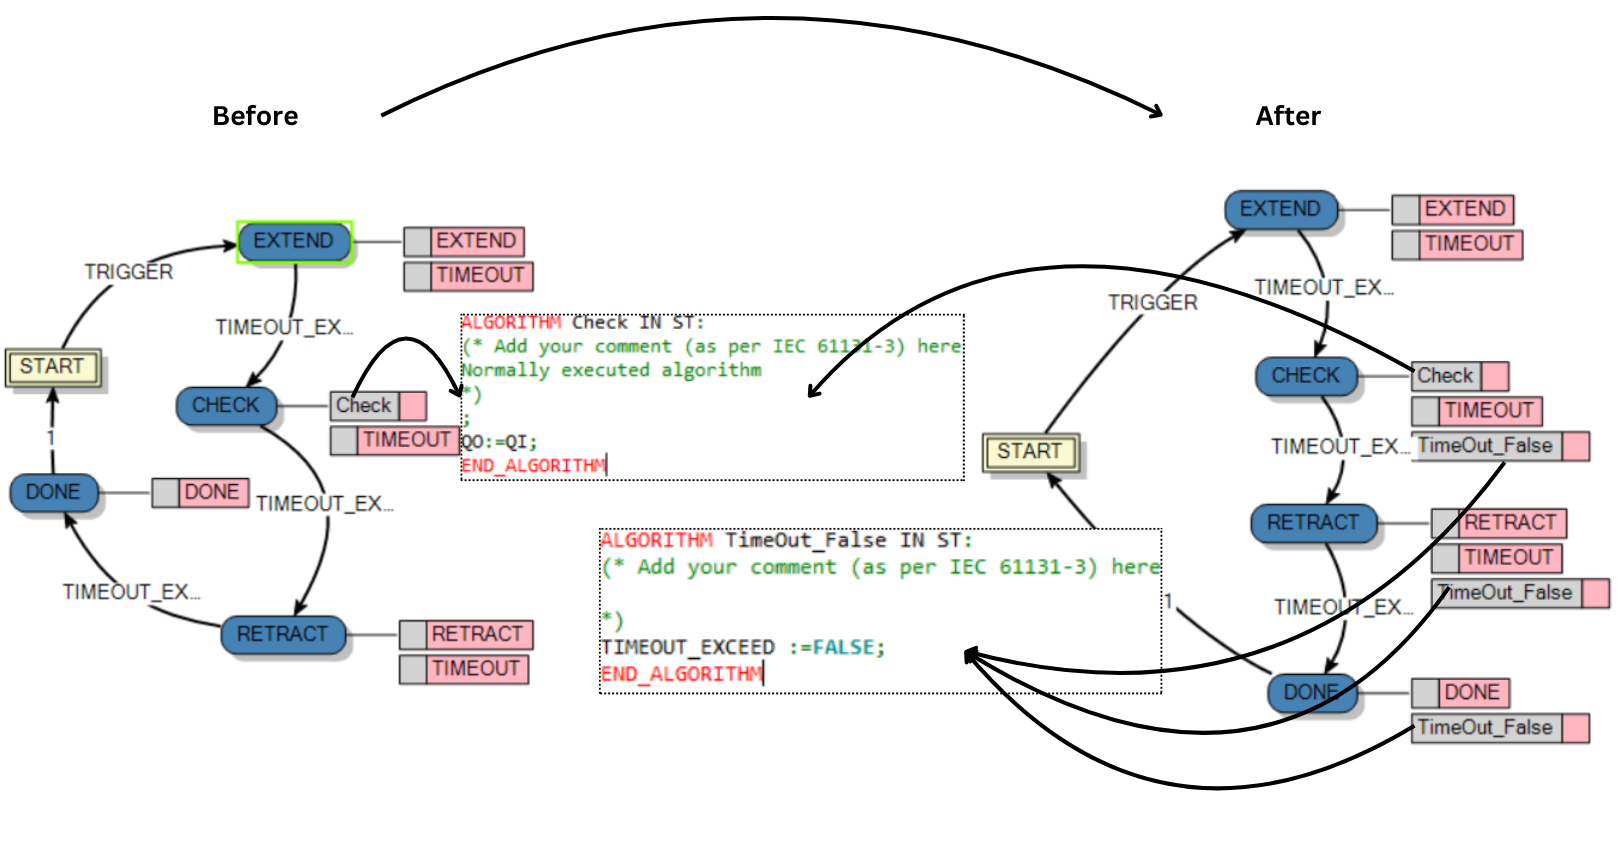
\includegraphics[width=0.99\linewidth]{MX_Papers/Paper10/Figures/SemanticExexcissue.png}
    \caption{Semantic Execution Issue: Illustration of how different runtime environments handle identical events differently, leading to unexpected behavior in ported applications.}
    \label{fig:semantic_issue}
\end{figure}

The primary semantic difference identified was in how EAE handles sequences of identical events. Unlike the IEC 61499 standard specification, EAE adopts a specific semantic execution model where a single event trigger can result in a direct transition to the final state, bypassing intermediate states entirely.

This semantic difference has significant implications for control applications, where applications developed on one platform may not function correctly on another, timing-dependent logic may behave unexpectedly, safety-critical functions may not operate as intended, and debugging becomes more complex due to platform-specific behavior.

The identification of these semantic differences demonstrates the critical importance of cross-platform testing in ensuring the reliability and safety of IEC 61499 applications.

\subsection{Portability Issues and Solutions}

The case study identified several specific portability issues that arise when moving IEC 61499 applications between different development and runtime environments:

\begin{enumerate}
    \item \textbf{Standard Function Block Compatibility}: Composite function blocks containing standard function blocks (such as E\_DELAY) cannot be directly imported into some platforms due to pre-compiled nature of standard blocks.
    
    \item \textbf{Namespace and Adapter Issues}: Adapters may not be located unless the correct namespace is specified, and composite function blocks involving adapters may require manual connection redrawing.
    
    \item \textbf{Algorithm Format Differences}: Algorithm sections may contain duplicate statements or case sensitivity issues that require manual correction.
    
    \item \textbf{Naming Convention Conflicts}: Algorithm names containing certain character sequences may not be supported across all platforms.
\end{enumerate}

These issues highlight the need for systematic approaches to portability validation and the importance of comprehensive testing across multiple platforms.

\subsection{Framework Evaluation Results}

The evaluation of the cross-platform testing framework demonstrated its effectiveness in identifying portability issues and ensuring consistent behavior across different runtime environments. The framework successfully generated comprehensive test applications from service sequence models, identified semantic execution differences between platforms, detected implementation bugs in ported applications, provided automated validation of function block behavior, and reduced manual effort required for cross-platform testing.

The evaluation results showed that the framework could detect both expected and unexpected behavioral differences, providing valuable feedback for developers working with multiple IEC 61499 platforms.

\section{Challenges and Limitations}

While the cross-platform testing methodologies provide significant benefits for IEC 61499 application development, several challenges and limitations must be acknowledged and addressed.

\subsection{Vendor-Specific Implementation Variations}

The primary challenge in cross-platform IEC 61499 development is the significant variation in how different vendors implement the standard. These variations can occur at multiple levels including syntax interpretation, where different vendors may interpret the XML format differently; semantic implementation, where execution semantics may vary significantly between platforms; feature support, where not all platforms support the complete set of IEC 61499 features; and performance characteristics, where timing and performance may vary between platforms.

These variations make it difficult to create truly portable applications and require comprehensive testing across all target platforms.

\subsection{Timing and Performance Considerations}

The current testing framework focuses primarily on event-based behavior and does not address timing verification. This limitation is significant for real-time control applications where timing is critical for proper operation. Different platforms may process events at different rates, and the time required to execute algorithms may vary significantly between runtime environments. Network communication timing may also differ between platforms, and meeting real-time constraints may be more challenging on some platforms than others. These timing-related challenges must be addressed in future work to provide more comprehensive validation of IEC 61499 applications.

\subsection{Scalability and Industrial Applicability}

The current testing framework has been validated primarily with academic and research-oriented case studies. The scalability to large-scale industrial applications remains to be demonstrated. Large applications may require extensive test suites that could take significant time to execute and may require substantial computational resources. Additionally, keeping test suites current with application changes presents ongoing maintenance overhead. The availability of industrial-scale function block libraries for testing is limited, making it difficult to validate the approach with real-world applications.

\subsection{Integration with Development Workflows}

The integration of cross-platform testing into existing development workflows presents additional challenges that must be addressed to ensure widespread adoption. Seamless integration with existing development tools is essential for practical implementation. Developers must learn new testing methodologies, which may require significant training and adaptation. Development processes may need to be modified to accommodate the new testing approaches, and additional resources may be required for testing activities. These challenges must be carefully managed to ensure successful adoption of cross-platform testing methodologies in industrial practice.

\section{Conclusion}

The development of comprehensive cross-platform testing methodologies for IEC 61499 function blocks addresses a critical need in industrial automation systems. The research presented in this chapter demonstrates that systematic approaches to testing and validation can significantly improve the portability and reliability of IEC 61499 applications.

The key contributions of this work include the development of comprehensive test function blocks for testing data types, boundary conditions, standard functions, and adapter support. The research also presents systematic model-based testing methodologies using service sequence models for test specification and automated generation. Additionally, the work demonstrates the creation of cross-platform test applications that can execute across different IEC 61499 runtime environments, along with real-world validation through industrial case studies. The systematic identification and documentation of platform-specific execution differences represents another significant contribution to the field.

The case study results demonstrate that cross-platform testing can identify significant behavioral differences between IEC 61499 platforms, highlighting the importance of comprehensive validation before deploying applications to production environments.

Future work should focus on extending the framework to address timing and performance considerations, testing with large-scale industrial applications, improving integration with existing development workflows, further automation of the testing process, and contributing to the development of standardized testing approaches.

The methodologies presented in this chapter provide a foundation for improving the reliability and portability of IEC 61499 applications, contributing to the broader goal of achieving truly interoperable industrial automation systems.
